\section{正定核的构造}
\label{sec:rkhs-kernel-constructions}

定理~\ref{thm:rkhs-moore-aronszajn}把问题归结为核的正定性，但直接检验一个二元函数的正定性并不方便：定义要求对一切有限点组和一切系数核验二次型。本节给出三条可操作的规则：把核写成特征向量的内积；对已知正定核作非负线性组合；对已知正定核作逐点乘积。每条规则都回到有限Gram矩阵的二次型来核验，最后用它们验证多项式核与高斯核。

\subsection{特征映射构造}
\label{sec:rkhs-feature-maps}

最常用的验证办法是把输入映到一个内积空间，再用像的内积定义核。二次型于是变成一个向量的长度平方，自然非负。

\begin{definition}[特征映射]
\label{def:rkhs-feature-map}
设$X$是非空集合，$\mathcal F$是Hilbert空间，$\Phi:X\to\mathcal F$是任意映射。称
\[
K(x,y)=\langle\Phi(x),\Phi(y)\rangle_{\mathcal F}\qquad(x,y\in X)
\]
为由$\Phi$给出的核，称$\Phi$为$K$的一个\term{特征映射}（feature map），$\mathcal F$为相应的特征空间（feature space）。
\end{definition}

由特征映射给出的核总是正定的：对任意点组与系数，
\[
\sum_{i,j}\overline{c_i}\,c_j\,K(x_i,x_j)=\Bigl\langle\sum_ic_i\Phi(x_i),\ \sum_jc_j\Phi(x_j)\Bigr\rangle_{\mathcal F}=\Bigl\lVert\sum_jc_j\Phi(x_j)\Bigr\rVert_{\mathcal F}^2\geq0 ,
\]
共轭对称性则来自内积本身。用矩阵写，若$\mathcal F=\mathbb K^d$，记$\bm\Phi$为第$i$行是$\Phi(x_i)^*$的$n\times d$矩阵，则Gram矩阵是$\bm\Phi\bm\Phi^*$。

反过来，每个正定核都有特征映射：取$\mathcal F=H_K$，$\Phi(x)=K_x$，则$\langle K_x,K_y\rangle_{H_K}=K(x,y)$。称它为\term{规范特征映射}（canonical feature map）。所以“$K$正定”与“$K$有某个特征映射”是等价的两种说法。

\paragraph{线性核与有限特征核}

在$\mathbb R^d$上，取$\Phi(\bm x)=\bm x$，得到\term{线性核}（linear kernel）$K(\bm x,\bm y)=\bm x^{\top}\bm y$。在$\mathbb R$上，展开平方可得
\[
(1+xy)^2=1+2xy+x^2y^2=\bigl\langle(1,\sqrt2\,x,x^2),\ (1,\sqrt2\,y,y^2)\bigr\rangle ,
\]
所以二次多项式核是三维特征向量的内积核。这类由有限个特征分量给出的核称为有限特征核，它们的Gram矩阵秩不超过特征维数，因而在点数超过特征维数时一定奇异。

\paragraph{特征维数与RKHS}

同一个核可以有许多不同的特征映射。仿射核$1+xy$既可以由$\Phi_1(x)=(1,x)\in\mathbb R^2$给出，也可以由$\Phi_2(x)=(1,x/\sqrt2,x/\sqrt2)\in\mathbb R^3$给出，因为$1+\tfrac{xy}{2}+\tfrac{xy}{2}=1+xy$。特征空间的维数和坐标都不同，核却相同，由核确定的RKHS也相同。所以特征维数不是空间的性质，RKHS中的函数及其范数要从核读出。

下面说明怎样从任何一个特征映射读出RKHS。给定$\Phi:X\to\mathcal F$，每个参数$w\in\mathcal F$确定一个函数
\[
f_w(x)=\langle\Phi(x),w\rangle_{\mathcal F}.
\]
令$V$为$\{\Phi(x):x\in X\}$张成的闭子空间，$P_V$为到$V$的正交投影。$w-P_Vw$与每个$\Phi(x)$正交，所以$f_w=f_{P_Vw}$：$V^\perp$中的参数分量对函数没有任何影响。

\begin{theorem}[特征映射给出的RKHS]
\label{thm:rkhs-feature-space}
设$\Phi:X\to\mathcal F$是正定核$K$的特征映射，$V$为$\Phi(X)$张成的闭子空间。则
\begin{equation*}
\begin{gathered}
H_K=\{f_w:w\in\mathcal F\},\\
\lVert f_w\rVert_{H_K}=\lVert P_Vw\rVert_{\mathcal F}=\min\{\lVert u\rVert_{\mathcal F}:u\in\mathcal F,\ f_u=f_w\} ,
\end{gathered}
\end{equation*}
并且$w\mapsto f_w$限制在$V$上是从$V$到$H_K$的等距同构。
\end{theorem}

\begin{proof}
线性映射$A:w\mapsto f_w$的核是$\{w:\langle\Phi(x),w\rangle=0,\ \forall x\}=V^\perp$，所以$A$在$V$上是单射，且$A(\mathcal F)=A(V)$。令$H=A(\mathcal F)$，规定$\langle Aw,Au\rangle_H=\langle P_Vw,P_Vu\rangle_{\mathcal F}$，则$A|_V$是等距同构，$H$作为闭子空间$V$的等距像是Hilbert空间，运算是逐点的。

令$k_x=A\Phi(x)$。因$\Phi(x)\in V$，有$\langle k_x,f_w\rangle_H=\langle\Phi(x),P_Vw\rangle=\langle\Phi(x),w\rangle=f_w(x)$；而$k_x(y)=\langle\Phi(y),\Phi(x)\rangle=K(y,x)$，即$k_x=K_x$。所以$H$是以$K$为再生核的RKHS，由定理~\ref{thm:rkhs-moore-aronszajn}的唯一性，$H=H_K$。最后，$f_u=f_w$当且仅当$u-w\in V^\perp$，此时$P_Vu=P_Vw$，而$\lVert u\rVert\geq\lVert P_Vu\rVert$，等号在$u\in V$时取得。
\end{proof}

定理的最后一个等式说明：在冗余的特征表示中，任意一个能给出$f$的参数，其长度只是$\lVert f\rVert_{H_K}$的上界；只有落在$V$中的参数，长度才等于函数的范数。

\begin{example}[冗余特征]
\label{ex:rkhs-redundant-features}
取$\Phi(x)=(x,x)\in\mathbb R^2$，核为$K(x,y)=2xy$。$V$是直线$\operatorname{span}\{(1,1)\}$，正交补方向是$(1,-1)$。参数$(2,0)$、$(1,1)$、$(0,2)$都给出同一函数$f(x)=2x$，长度分别为$2$、$\sqrt2$、$2$；由定理~\ref{thm:rkhs-feature-space}，$\lVert f\rVert_{H_K}=\sqrt2$，是$(2,0)$在$V$上的投影$(1,1)$的长度，见图~\ref{fig:rkhs-visible-parameters}。

直接核对：$H_K$由$f(x)=cx$组成，核截面$K_x(t)=2xt$，再生性质要求$\langle 2xt,ct\rangle=cx$，故$\langle at,ct\rangle_{H_K}=ac/2$，$\lVert 2x\rVert_{H_K}^2=4/2=2$，结果一致。特征空间是二维的，RKHS却是一维的。
\end{example}

\begin{figure}[!htb]
  \centering
  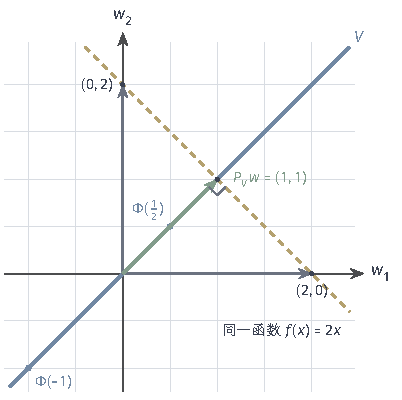
\includegraphics[width=68.1mm]{figures/02-abstract-mathematics/03-function-spaces/tikz/c5-visible-parameters/figure.pdf}
  \caption{冗余特征$\Phi(x)=(x,x)$的参数平面。各点的特征$\Phi(x)$都落在蓝色直线$V$上；黄色虚线上的参数都给出同一函数$f(x)=2x$。其中与$V$相交的$P_Vw=(1,1)$长度最短，为$\sqrt2$，这就是$\lVert f\rVert_{H_K}$；$(2,0)$与$(0,2)$长度为$2$，多出的部分来自对函数没有影响的$V^\perp$方向。}
  \label{fig:rkhs-visible-parameters}
\end{figure}

对仿射核的两个特征映射，$\Phi_1$的$V$是整个$\mathbb R^2$，所以$\lVert a+bt\rVert_{H_K}^2=a^2+b^2$，与第~\ref{sec:rkhs-evaluation-bounds}节一致。$\Phi_2$的$V$是$\operatorname{span}\{(1,0,0),(0,1,1)/\sqrt2\}$，参数$(a,b/\sqrt2,b/\sqrt2)$给出$a+bt$，长度同样是$\sqrt{a^2+b^2}$；参数$(a,\sqrt2\,b,0)$也给出同一函数，长度$\sqrt{a^2+2b^2}$却更大。

\subsection{非负线性组合}
\label{sec:rkhs-nonnegative-combinations}

特征映射适合验证可以写成内积的核。更多的核由几个已知核组合得到，只要组合方式保持正定性，就不必为每个新核重新寻找特征映射。最简单的组合是加权求和。

\begin{theorem}[非负线性组合]
\label{thm:rkhs-nonnegative-combination}
设$K_1,\ldots,K_m$是$X$上的正定核，$\alpha_1,\ldots,\alpha_m\geq0$是非负实数。则$K=\sum_l\alpha_lK_l$是$X$上的正定核。
\end{theorem}

\begin{proof}
固定点组与系数向量$\bm c$，记$\bm G_l$为$K_l$的Gram矩阵，则$K$的Gram矩阵是$\sum_l\alpha_l\bm G_l$，且
\[
\bm c^*\Bigl(\sum_l\alpha_l\bm G_l\Bigr)\bm c=\sum_l\alpha_l\,\bm c^*\bm G_l\bm c\geq0 ,
\]
因为每一项都是非负数与非负数之积。实数情形下对称性显然保持。
\end{proof}

用特征映射表达，若$\Phi_l$是$K_l$的特征映射，把$\sqrt{\alpha_l}\,\Phi_l(x)$依次拼接成直和空间$\mathcal F_1\oplus\cdots\oplus\mathcal F_m$中的一个向量，其内积正是$\sum_l\alpha_lK_l(x,y)$。例如仿射核$1+xy$是常数核$1$（特征为常数$1$）与线性核$xy$之和，拼接特征就是前面的$\Phi_1(x)=(1,x)$。

系数的符号不能任意改变。仿射核减去常数核$2$得到$xy-1$，它在$x=y=0$处的值为$-1$；而正定核在单点上的Gram矩阵是$1\times1$矩阵$[K(x,x)]$，必须非负。所以两个正定核之差一般不是正定核。复系数同样不行：$\mathrm iK$的对角值是纯虚数，二次型不再取实值。

\subsection{逐点乘积}
\label{sec:rkhs-pointwise-products}

第二种组合是逐点相乘。这时乘积核的Gram矩阵是两个Gram矩阵的逐元素乘积，正定性来自卷二的Schur乘积定理：两个同阶Hermite半正定矩阵的逐元素乘积仍是Hermite半正定矩阵，可参考\BookChapterRef{chap:normed-inner-product-spaces}{卷二第3章“赋范空间与内积空间”}。其机制是把两组向量的内积相乘，等于它们张量积之间的内积。

\begin{theorem}[逐点乘积]
\label{thm:rkhs-pointwise-product}
设$K_1,K_2$是同一集合$X$上的正定核。则$K(x,y)=K_1(x,y)K_2(x,y)$是$X$上的正定核。若$\Phi_1,\Phi_2$分别是$K_1,K_2$取值于$\mathbb K^{d_1},\mathbb K^{d_2}$的特征映射，则$\Phi_1(x)\otimes\Phi_2(x)\in\mathbb K^{d_1d_2}$是$K$的特征映射。
\end{theorem}

\begin{proof}
固定点组，$K$的Gram矩阵是$\bm G_1\odot\bm G_2$，由Schur乘积定理它是Hermite半正定矩阵，所以$K$正定。对特征映射，按坐标展开$\langle u\otimes v,u'\otimes v'\rangle=\sum_{k,l}\overline{u_kv_l}\,u_k'v_l'=\langle u,u'\rangle\langle v,v'\rangle$，取$u=\Phi_1(x)$、$v=\Phi_2(x)$、$u'=\Phi_1(y)$、$v'=\Phi_2(y)$即得。
\end{proof}

\paragraph{两条辅助规则}

验证常见的连续核，还需要两条与乘积相关的简单规则。第一条是函数缩放：对任意$g:X\to\mathbb K$，$g(x)\overline{g(y)}$是正定核，因为
\[
\sum_{i,j}\overline{c_i}\,c_j\,g(x_i)\overline{g(x_j)}=\Bigl\lvert\sum_i\overline{c_i}\,g(x_i)\Bigr\rvert^2\geq0 ;
\]
于是由定理~\ref{thm:rkhs-pointwise-product}，$g(x)\overline{g(y)}K(x,y)$对任意正定核$K$仍正定。第二条是逐点极限：若正定核$K^{(k)}$在每个$(x,y)$处收敛到$K(x,y)$，则$K$正定，因为每个有限二次型都是非负数的极限。

\paragraph{多项式核与高斯核}

由这几条规则可以验证常用的核。常数$c\geq0$是以$\sqrt c$为特征的核，所以$c+\bm x^{\top}\bm y$正定（定理~\ref{thm:rkhs-nonnegative-combination}），它的$p$次幂即\term{多项式核}（polynomial kernel）$(c+\bm x^{\top}\bm y)^p$也正定（定理~\ref{thm:rkhs-pointwise-product}反复使用）。

$\mathbb R^d$上的高斯核$K_\sigma(\bm x,\bm y)=\exp\bigl(-\lVert\bm x-\bm y\rVert_2^2/(2\sigma^2)\bigr)$分三步验证。先展开指数中的平方：
\[
\exp\Bigl(-\frac{\lVert\bm x-\bm y\rVert_2^2}{2\sigma^2}\Bigr)
=g(\bm x)\,g(\bm y)\,\exp\Bigl(\frac{\bm x^{\top}\bm y}{\sigma^2}\Bigr),\qquad
g(\bm x)=\exp\Bigl(-\frac{\lVert\bm x\rVert_2^2}{2\sigma^2}\Bigr).
\]
再看中间因子：部分和$\sum_{k=0}^N(\bm x^{\top}\bm y)^k/(k!\,\sigma^{2k})$是线性核各次幂的非负组合，因而正定；指数级数逐点收敛，由逐点极限规则，$\exp(\bm x^{\top}\bm y/\sigma^2)$正定。最后由函数缩放规则乘上$g(\bm x)g(\bm y)$。这样得到的是正定性；严格正定性是更强的性质，第~\ref{sec:rkhs-pd-kernels}节已经说明它需要另外的论证。

\paragraph{运算在核截面上的效果}

核的运算直接作用在核截面上：和核的截面是两个截面之和，乘积核的截面是两个截面之积。图~\ref{fig:rkhs-kernel-operations}在$x=0.4$处比较仿射核与高斯核（$\sigma=0.3$）。和核的截面在仿射趋势上叠加了一个局部隆起；乘积核的截面仍集中在$x$附近，但被仿射因子$1+0.4t$拉得右高左低。所以乘积核对应空间中的函数同时带有两种核的特点：局部性来自高斯因子，倾斜来自仿射因子。

\begin{figure}[!htb]
  \centering
  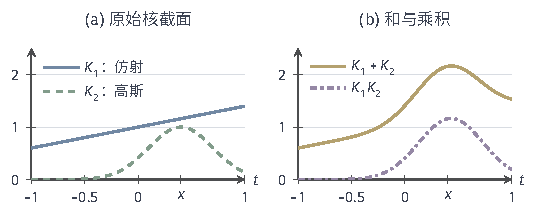
\includegraphics[width=90.7mm]{figures/02-abstract-mathematics/03-function-spaces/tikz/c5-kernel-operations/figure.pdf}
  \caption{核运算在核截面上的效果，固定$x=0.4$，$t\in[-1,1]$。(a)~仿射核截面$1+0.4t$与高斯核截面（$\sigma=0.3$）；(b)~两者之和与逐点乘积。和核的截面是两个截面相加，乘积核的截面是两个截面相乘，仍保持以$x$为中心的局部形状。}
  \label{fig:rkhs-kernel-operations}
\end{figure}

本节的规则都从已知的核或已知的特征出发。还有一种重要的特征来自核本身的谱：在定义域上加入测度后，核积分算子的特征函数给出一组按特征值加权的特征，这要用到算子的谱理论，在第~\ref{sec:rkhs-mercer}节另行构造。
